\documentclass[a4paper,12pt]{article} 

%%% Работа с русским языком
\usepackage{cmap}                           % поиск в PDF
\usepackage{mathtext} 			 	       % русские буквы в формулах
\usepackage[T2A]{fontenc}               % кодировка
\usepackage[utf8]{inputenc}              % кодировка исходного текста
\usepackage[english,russian]{babel}  % локализация и переносы
\usepackage[left=2cm,right=2cm,
    top=2cm,bottom=2cm,bindingoffset=0cm]{geometry}
\usepackage{wrapfig}
\usepackage{gensymb}
\usepackage{textcomp}
\usepackage{multirow}
\usepackage{amsmath,amsfonts,amssymb,amsthm,mathtools} % AMS
\usepackage{euscript}	 % Шрифт Евклид
\usepackage{mathrsfs} % Красивый матшрифт
\usepackage{graphicx}%Вставка картинок правильная
\usepackage{float}%"Плавающие" картинки
\usepackage{wrapfig}%Обтекание фигур (таблиц, картинок и прочего)
\title{Лабораторная работа 3.2.4 

Свободные колебания в электрическом контуре}
\author{Кагарманов Радмир Б01-106}
\date{14 сентября 2022 г.}

\begin{document}
\maketitle
\thispagestyle{empty}
\newpage
\setcounter{page}{1}
\paragraph{Цель работы:} исследование свободных колебаний в электрическом колебательном контуре.
\paragraph{В работе используется:} генератор импульсов, электронное реле, магазин сопротивлений, магазин ёмкостей, катушка индуктивности, электронный осциоллограф, универсальный измерительный мост.
\paragraph{Экспериментальная установка\\}

\begin{figure}[!h]
\centering
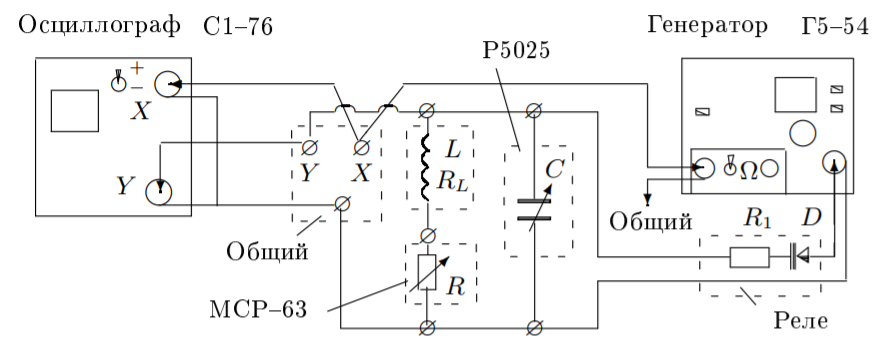
\includegraphics[width=0.9\linewidth]{Установка.png}
\caption{Экспериментальная установка}
\label{fig:mpr}
\end{figure}

На рис. 1 приведена схема установки для исследования свободных колебаний в контуре, содержащем постоянную индуктивность $L$ с активным сопротивлением $R_{L}$, а также переменные сопротивление $R$ и ёмкость $C$, выбираемые из соответствующих магазинов. Картина колебаний напряжения на ёмкости наблюдается на экране двухканального осциоллографа. Выходные разъёмы схемы и входы каналов осциоллографа собраны на отдельной панели $\text{П}$. \par
Для периодического возбуждения колебаний в контуре используется генератор импульсов. С выхода генератора сигналы поступают на колебательный контур через электронное реле, которое содержит диодный тиристор и ограничительный резистор.
\paragraph{Обработка результатов\\}
Измерим идуктивность $L$ и сопротивление $R_L$ катушки в зависимости от частоты.
\begin{table}[h!]
\begin{center}

\begin{tabular}{|c|c|c|}
\hline
$\nu$, Гц & $L$, мГн & $R_L$, Ом \\ \hline
50        & 139    & 20      \\ \hline
1000      & 134    & 28      \\ \hline
5000      & 135    & 48      \\ \hline
\end{tabular}
\caption{Некоторые параметры катушки индуктивности}
\end{center}
\end{table} \\ \\
\[L = 136\pm 2~ мГн\]
\subparagraph{1.}
В таблице 2 и на рис. 2 представлено сравнение экспериментальных значений периодов с теоретическими, которые считаются по формуле X:
\begin{equation}
    T=2\pi \sqrt{LC}
\end{equation}

\begin{table}[h!]
\begin{center}
\begin{tabular}{|c|c|c|c|c|c|c|}
\hline
С, мкФ & t, мс & $\sigma_t$, мс & $N$ периодов & $T_{prac}$, мс & $T_{theor}$, мс & $\sigma_T$, мс \\ \hline
0,02    & 5,00   & 0,25            & 5          & 0,33           & 0,33            & 0,02           \\ \hline
0,1    & 5,00   & 0,25           & 2           & 0,72           & 0,74           & 0,05           \\ \hline
0,2    & 5,00   & 0,25            & 4           & 1,03         & 1,05          & 0,07           \\ \hline
0,3    & 5,00   & 0,25            & 3         & 1,26           & 1,28            & 0,09           \\ \hline
0,4    & 5,00   & 0,25            & 5         & 1,44           & 1,48           & 0,10           \\ \hline
0,5    & 5,00   & 0,25            & 4         & 1,60           & 1,66            & 0,11           \\ \hline
0,6    & 5,00   & 0,25            & 4         & 1,75           & 1,81            & 0,12           \\ \hline
0,7    & 5,00   & 0,25            & 3          & 1,87           & 1,96            & 0,13           \\ \hline
\end{tabular}
\caption{Таблица данных измерения периода свободных колебаний и сравнение с теорией}
\end{center}
\end{table} 
\newpage
\begin{figure}[!h]
\centering
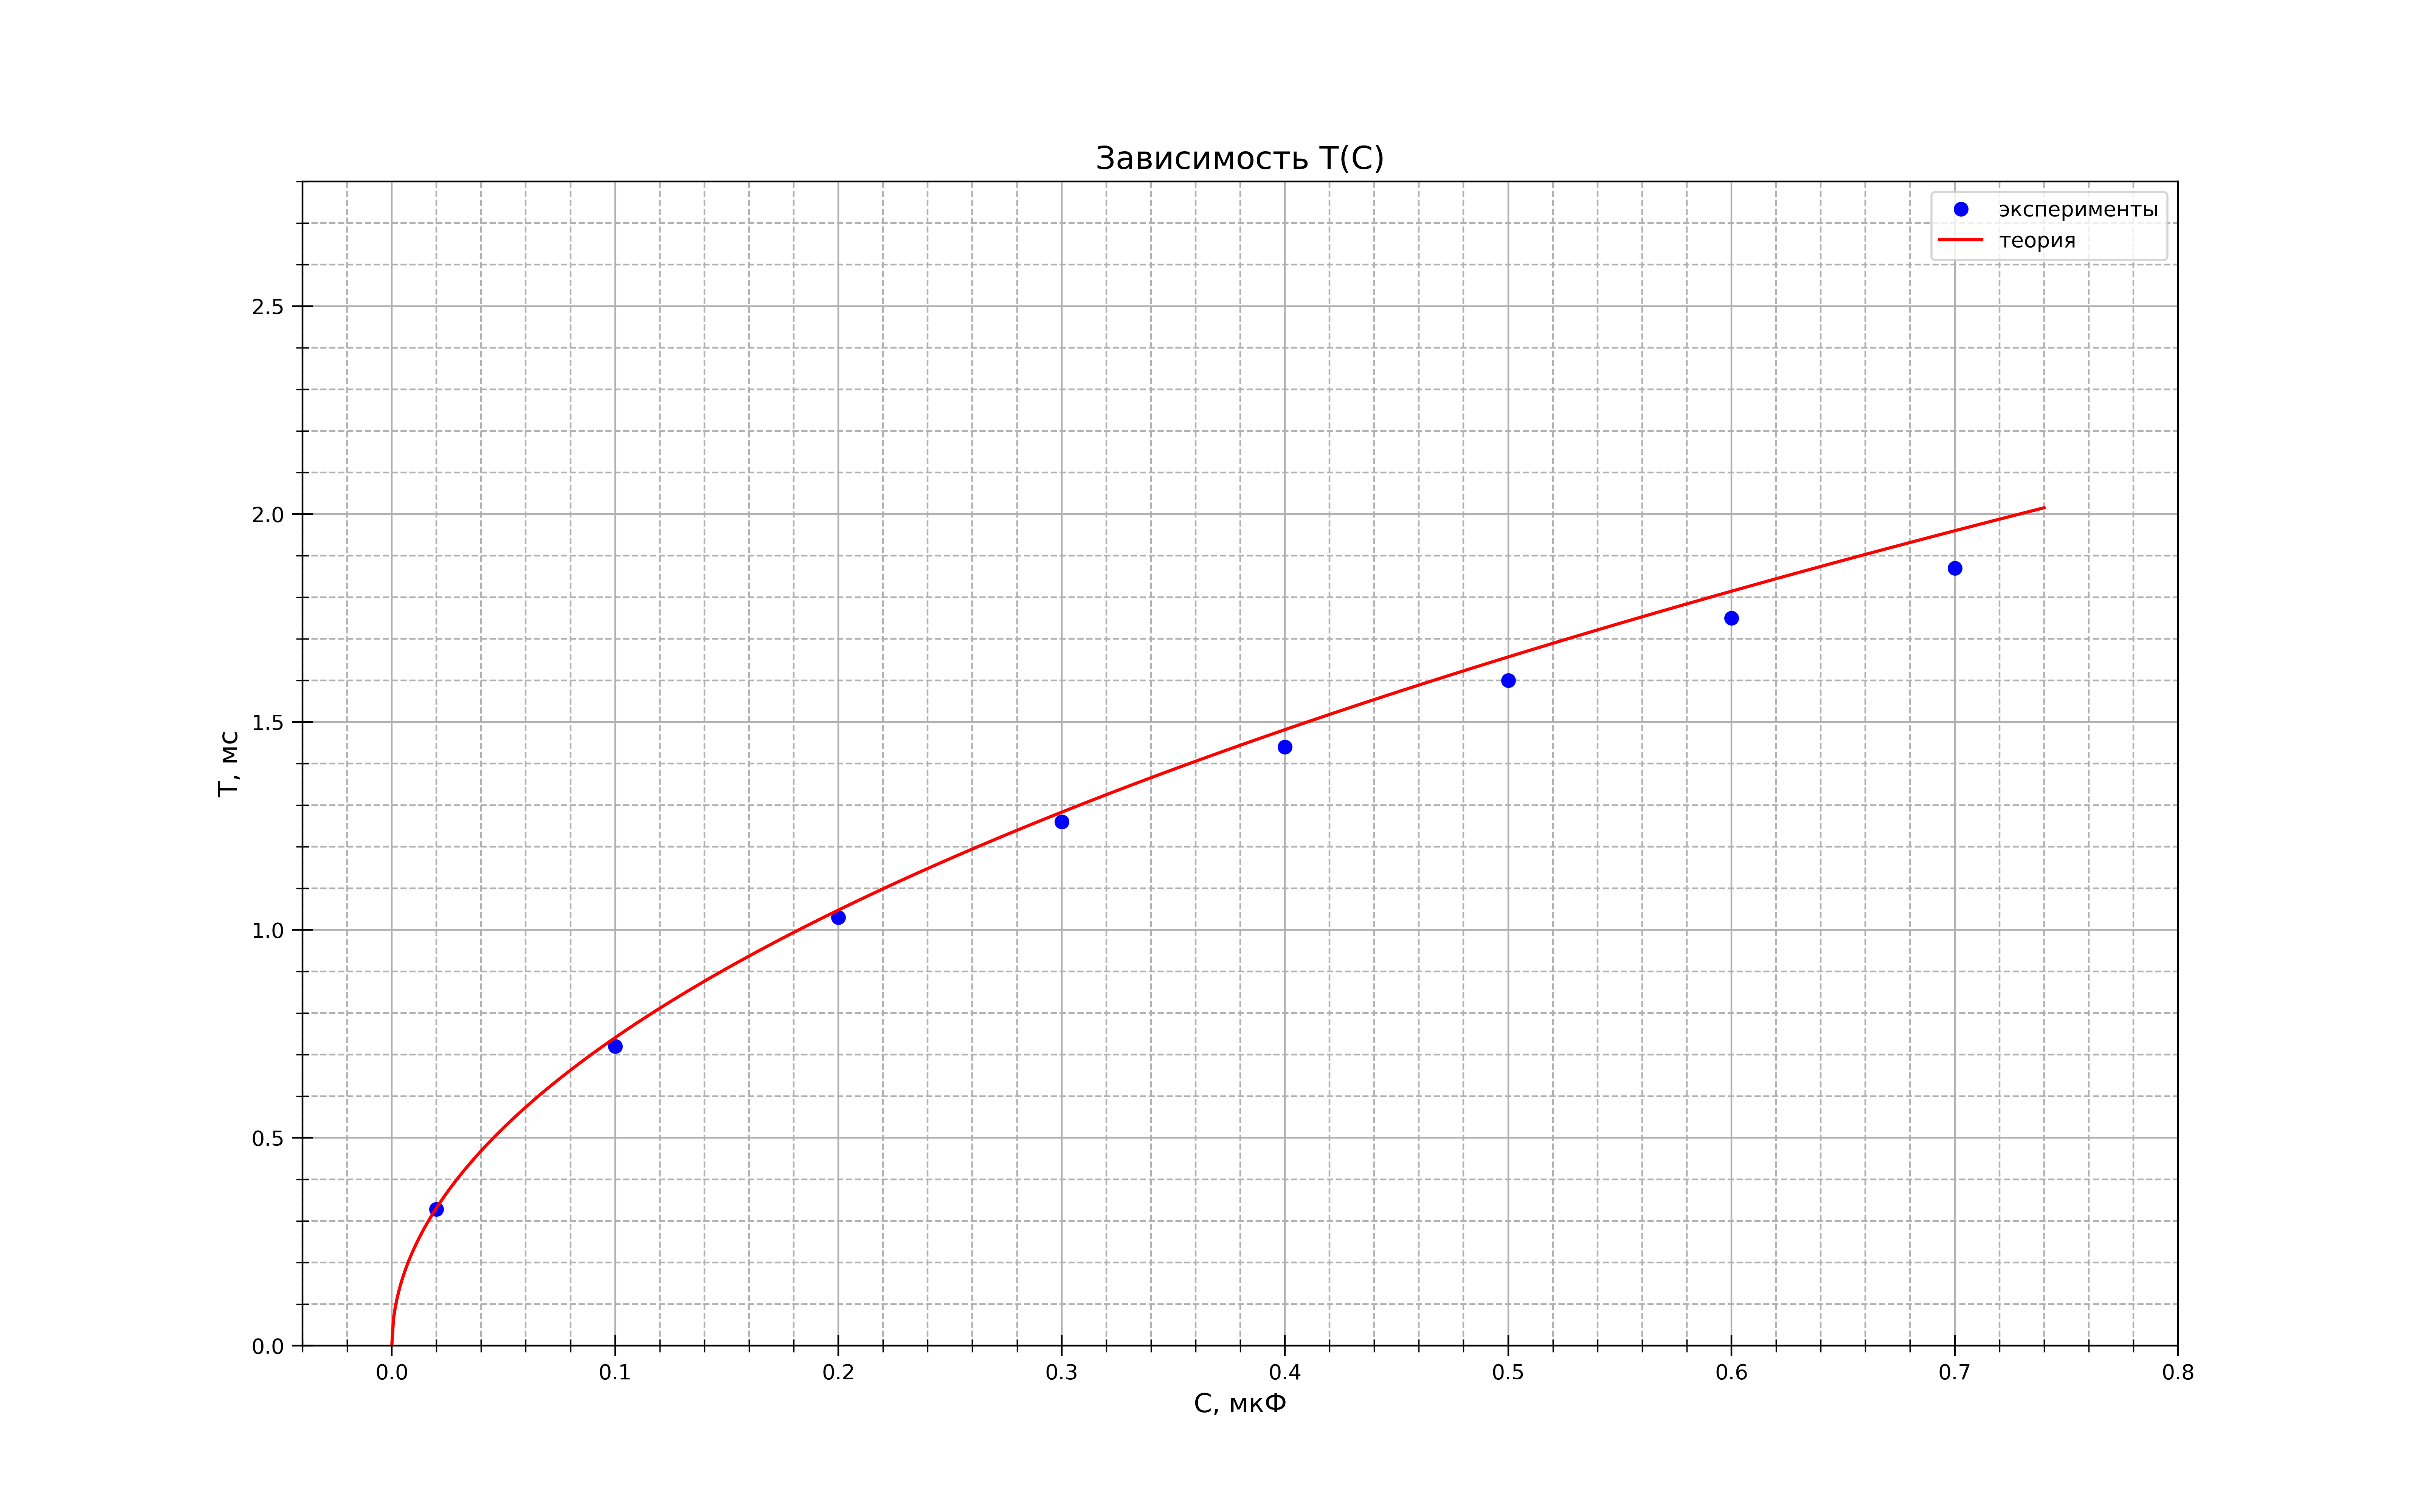
\includegraphics[width=0.9\linewidth]{graph1.png}
\caption{Зависимость T(C).}
\label{fig:mpr}
\end{figure}
Видим, что экспериментальные значения близки к теоретическим.
\subparagraph{2.} 
\[R_{крит} = 4\pi \nu_{0} L = 8,73 \text{кОм}\]
Для этих значений $L$ и $C$ рассчитаем декремент затухания для каждого сопротивления из интервала $(0,1-0,3)R_{крит}$. Из этих данных по формуле 
\[R_{крит} = R_{\Sigma} \sqrt{\left[\dfrac{2\pi}{\theta}\right]^2 + 1}\]
находим $R_{крит}$ запишем все в таблицу. 

\begin{table}[h!]
\begin{center}
\begin{tabular}{|c|c|c|c|c|c|c|c|c|}
\hline
R, Ом & $U_1$, дел & $\sigma_{U_1}$, дел & $U_2$, дел & $\sigma_{U_2}$, дел & $\theta$ & $\sigma_{\theta}$ & $R_{крит}$, Ом & $\sigma_{R_{crit}}$, Ом \\ \hline
700  & 6,66          & 0,33                 & 1,00        & 0,05                 & 0,474     & 0,034              & 9300          & 651                    \\ \hline
750  & 4,60          & 0,23                 & 1,00        & 0,05                 & 0,509     & 0,036              & 9283          & 650                    \\ \hline
1000  & 6,60          & 0,33                 & 0,90        & 0,05                 & 0,660     & 0,047              & 9567          & 670                    \\ \hline
1250  & 5,60          & 0,28                 & 1,00        & 0,05                 & 0,805      & 0,057               & 9831          & 688                    \\ \hline
1500  & 4,80          & 0,24                 & 0,60        & 0,03                 & 1,040      & 0,074               & 9181          & 643                    \\ \hline
1750  & 6,60          & 0,33                 & 0,60          & 0,03                 & 1,200      & 0,084               & 9324          & 653                    \\ \hline
\end{tabular}
\caption{Таблица измерения $R_{крит}$}
\end{center}
\end{table}
В итоге мы получаем $R_{крит}=9,414\pm 0,220~ \text{кОм}$.\\
Экспериментальный результат сильно отличается от теоретического. Скорее всего это из-за того, что в описании работы было написано, использовать $L\approx 200 ~\text{мГн}$ для подсчёта $R_{крит}$. А при измерении нашей катушки индуктивность получилась $L=139 ~\text{мГн}$. 
\subparagraph{3.}Рассмотрим свободные колебания на фазовой плоскости, для этого подключим место соединения катушки индуктивности и магазина сопротивлений к выходу $X$ и включим на осциллографе канал $X-Y$. В итоге мы получаем картинку на экране как на рисунке ниже.
\begin{figure}[h!]
\begin{center}
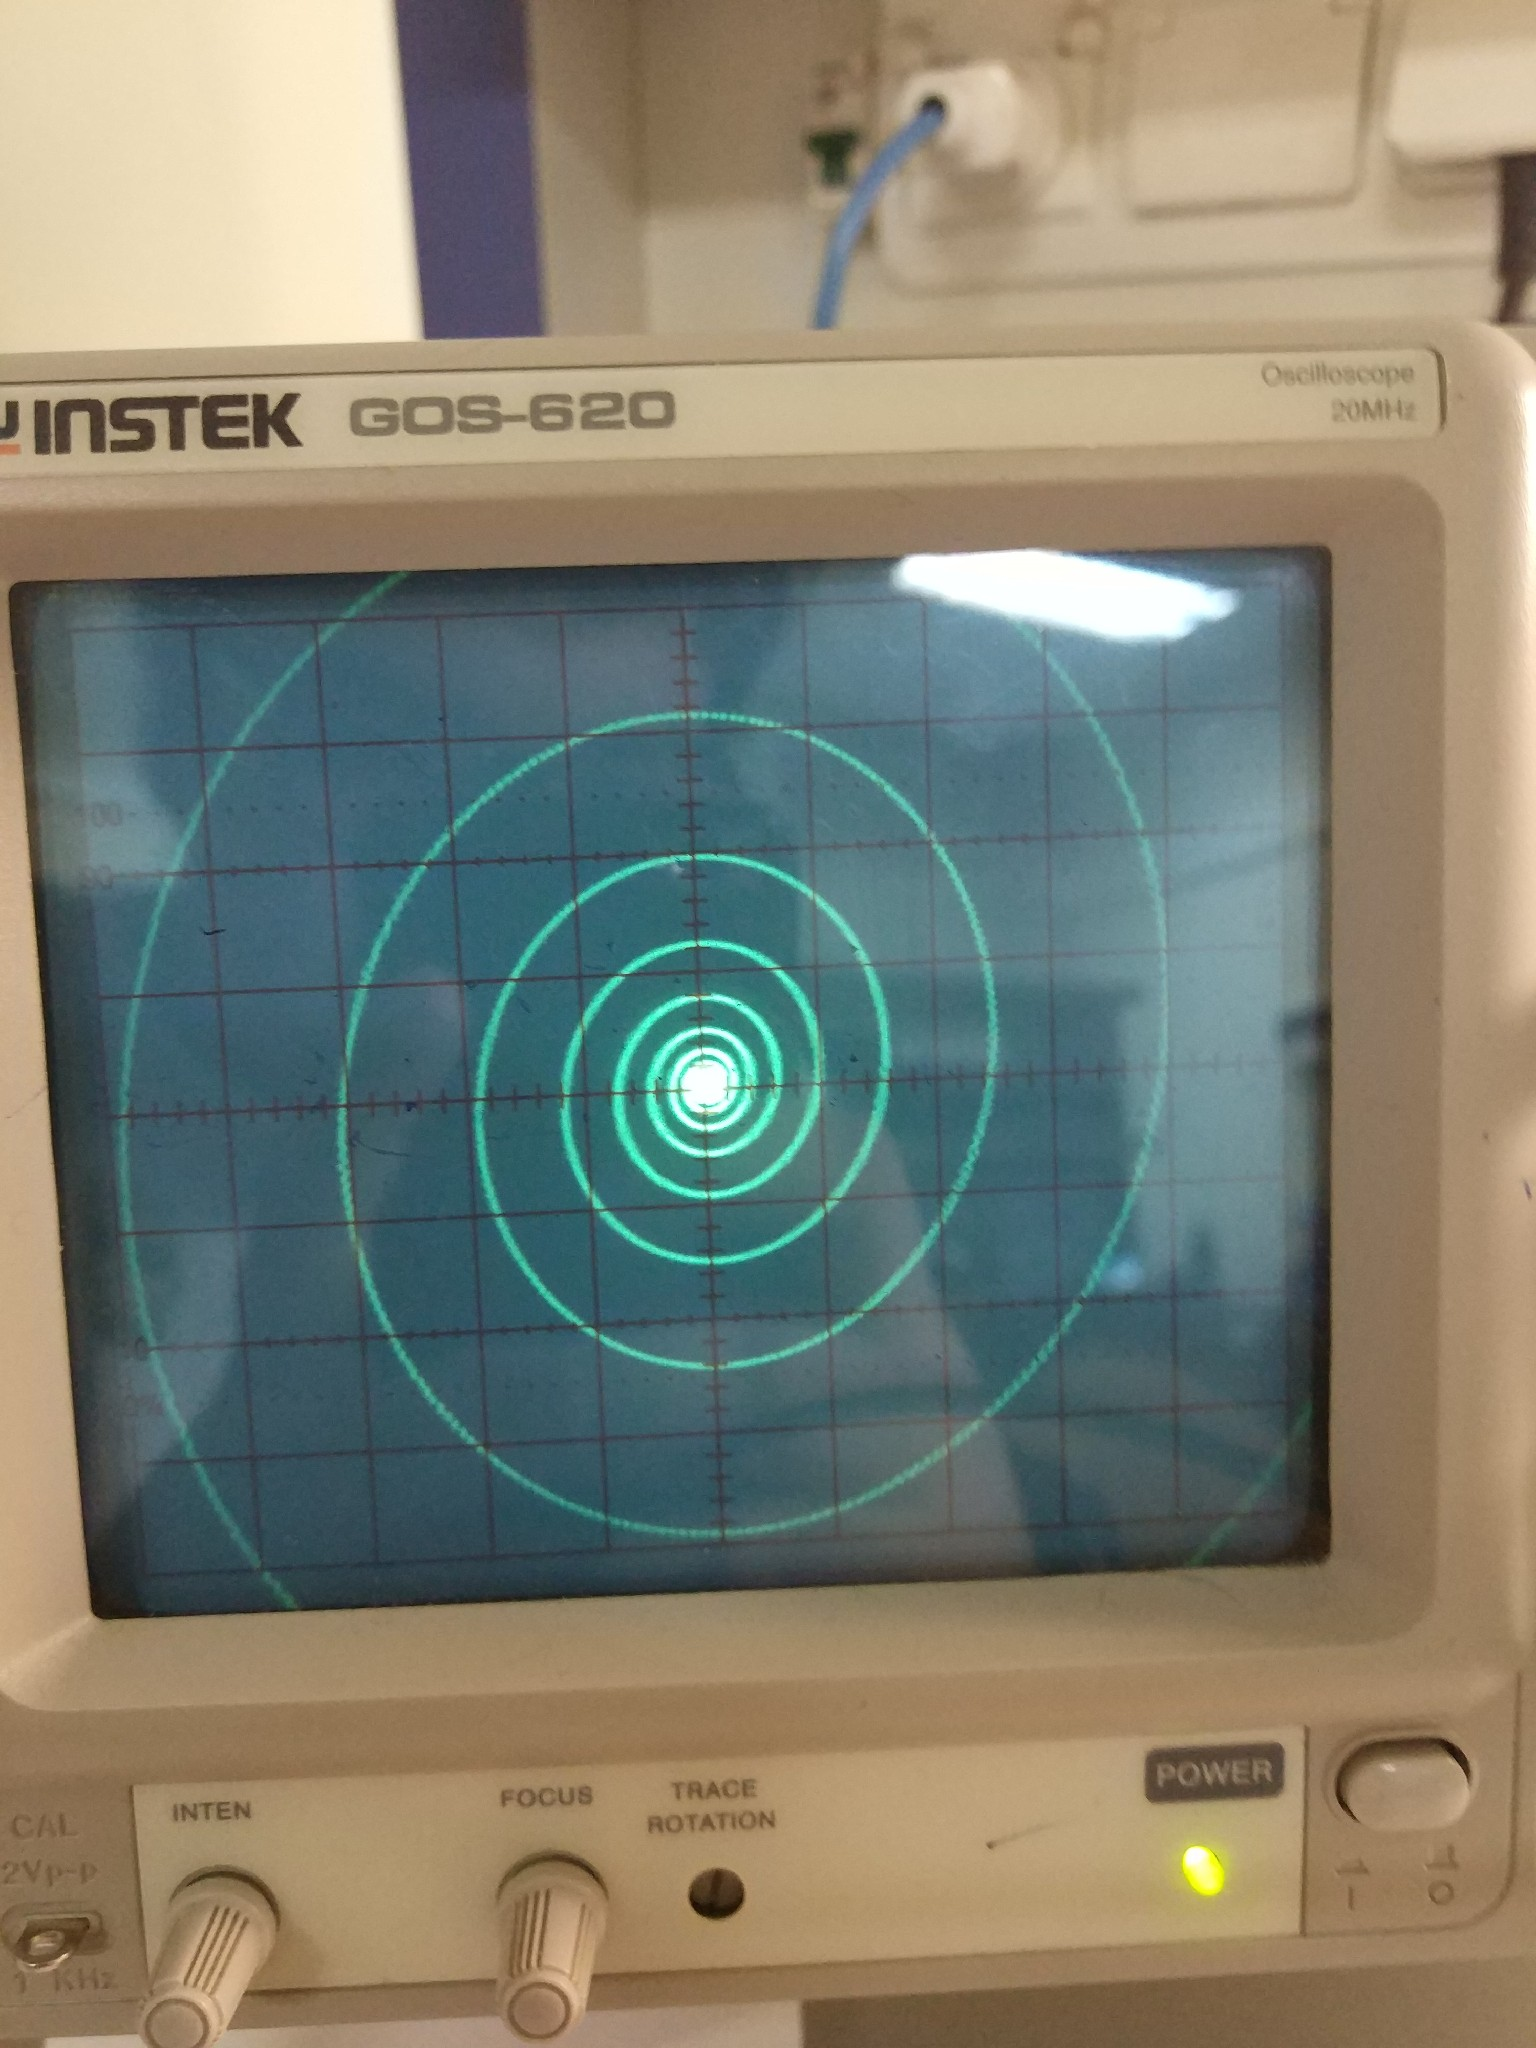
\includegraphics[width = 0.6\textwidth]{1.jpg}
\caption{Фазовая диаграмма для свободных колебаний}
\end{center}
\end{figure}
Для фазовой диаграммы для двух значений посчитаем так же декремент затухания

\begin{table}[h!]
\begin{center}
\begin{tabular}{|c|c|c|c|c|c|}
\hline
$R$, Ом &$U_1$, дел & $U_2$, дел & n & $\theta$ & $\sigma_{\theta}$ \\ \hline
750 & 0,6        & 3,9        & 4  & 0,468  & 0,033              \\ \hline
2150& 1          & 3,8        & 1  & 1,335     & 0,093              \\ \hline
\end{tabular}
\caption{Декремент затухания для фазовой диаграммы}
\end{center}
\end{table}
\subparagraph{4.}Добротность можно найти по формуле 
\[Q = \dfrac{\pi}{\theta}\]
Найдем ее для $R_{min} = 750$ Ом из графика и фазовой диаграммы. Итоговые результаты запишем в таблицу.

Так же добротность можно найти и из теоретических соображений по формуле
\[Q = \dfrac{1}{R}\sqrt{\dfrac{L}{C}}\]

Результаты так же занесем в таблицу, и в итоге мы получаем эту таблицу со всеми данными из данного эксперимента, по которой мы можем сравнить все полученные значения
\begin{table}[h!]
\begin{center}
\begin{tabular}{|c|c|c|c|c|c|c|c|}
\hline
\multirow{2}{*}{} & \multirow{2}{*}{$L_{coil}$, мГн} & \multicolumn{3}{c|}{$R_{crit}$, кОм}                         & \multicolumn{3}{c|}{Q}                 \\ \cline{3-8} 
                  &                                  & Теор.                 & Подбор              & Граф.          & Теор. & Граф.         & Спираль        \\ \hline
$R_{max}$         & \multirow{2}{*}{$136 \pm 2$}   & \multirow{2}{*}{8,73} & \multirow{2}{*}{9,36} & $9,28 \pm 0,65$ & 6,95   & $6,17 \pm 0,43$ & $6,71 \pm 0,47$  \\ \cline{1-1} \cline{5-8} 
$R_{min}$         &                                  &                       &                     & -    & - & - & - \\ \hline
\end{tabular}
\caption{Итоговые результаты эксперимента}
\end{center}
\end{table}
Мы не вычислили $\theta$ для $R=2150$ Ом через график и спираль. Для $R=750$ Ом видно, что спираль ближе к теории.
\paragraph{Вывод:} выполнив данную лабораторную работу, мы исследовали свободные колебания в электрическом контуре. Нашли $R_{крит}$, логарифмический декремент затухания $\theta$ и добротность $Q$ разными методами. Некоторые значения не сходятся с теорией.
\end{document}
